\section{Einführung}
\subsection{Wheatstonesche Brücke}
\subsection{Thermoelement}
\subsubsection{Seebeck-Effekt}
Unter dem Seebeck-Effekt versteht man das Auftreten einer Spannung zwischen zwei Leiterenden, wenn  längs des Leiters ein Temperaturgradient vorliegt. Die Spannung entsteht aus dem bestreben der Elektronen von dem wärmeren Enden, mit mehr kinetischer Energie, zu dem kälteren Ende mit einer höheren Elektronendichte zu kommen. Diese auftretende Spannung nennt sich Thermospannung und ist proportional zur Temperaturdifferenz der Leiterenden. Es gilt
\begin{equation}
\Delta U \sim \Delta T \Rightarrow \Delta U= \alpha_A\Delta T.
\end{equation} 
Der Faktor $\alpha_A$ heißt Seeeckkoeffizient. Dieser Effekt ist jedoch so nicht messbar, deswegen wird der Seeeckkoeffizient, wie in Abbildung \ref{fig:Thermoaufbau} dargestellt, bestimmt. Dies führt zu der Formel
\begin{equation}
\Delta U_{AB}=\alpha_A\cdot \Delta T -\alpha_B\cdot \Delta T = \alpha_{AB}\cdot \Delta T
\label{eq:Thermo}
\end{equation}
mit $\alpha_{AB}=\alpha_A-\alpha_B$.
\subsubsection{Peltier-Effekt}
Der Peltier-Effekt beschreibt die Umkehrung des Seebeck-Effekts, durch einen Aufbau ähnlich Abbildung \ref{fig:Thermoaufbau} wird nun ein konstanter Strom $I$ geleitet. Dabei kühlt sich ein Ende ab, während sich das andere erhitzt. Zwischen der umgesetzten Peltierwärme $\dot Q$ und dem Strom $I$ gilt
\begin{equation}
\dot Q = \pi_{AB}\cdot I \text{ mit } \pi_{AB}=\alpha_{AB}\cdot T.
\end{equation}
\section{Versuche}
\subsection{Wheatstonesche Brücke}
\subsection{Thermoelement}
Der Versuch wird wie in dem Schema \ref{fig:Thermoaufbau} aufgebaut und das Referenzbecken wird auf $T_2=1,6^\circ C$ mit Hilfe von Eiswasser gehalten. Nun wird das Becken 1 mit Hilfe einer Heizplatte erst bis auf $T_1=100^\circ C$ erhitzt und anschließend wieder auf die Ausgangstemperatur herunter gekühlt. Um den Abkühlprozess zu beschleunigen wird langsam Eis in das Becken 1 gegeben. Während des Aufwärmens und Abkühlens wird bei regelmäßigen Temperaturabständen die Spannung am Voltmeter bestimmt.
\begin{figure}[htbp] 
  \centering
	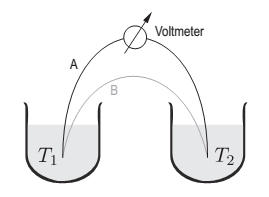
\includegraphics[width=0.7\textwidth]{Thermoaufbau.png}
	\caption{Schematische Darstellung des Thermoelemtsaufbau\footcite{anleitung-ws2014}}
  \label{fig:Thermoaufbau}
\end{figure}
\begin{figure}[H]
  \centering
  \begin{tikzpicture}
    \begin{axis}[
      width=15 cm,
      height=9 cm,
      xmin=0, xmax=105,
      ymin=0, ymax=5,
      xlabel={Differenz der beiden Probebecken $\Delta T$ [$^\circ K$]},
      ylabel={Gemessene Spannung $U$ [mV]},
      legend entries={Aufheitzprozess, Abkühlprozess, Linearer Fit beider Prozesse},
      legend pos=north west,
      domain=0.1:105,
    ]
      \addplot plot [only marks,mark=x,thick,error bars/.cd, x dir=both, x fixed=1, y dir=both, y fixed=0.1]  file {Tsteigend.txt};
      \addplot plot [only marks,mark=o,thick,error bars/.cd, x dir=both, x fixed=1, y dir=both, y fixed=0.1]  file {Tfallend.txt};
      \addplot[mark=none] {0.0361121*x};
    \end{axis}
  \end{tikzpicture}
  \caption{Gemessene Spannung gegen Differenz der Temperatur der Probebecken}
  \label{fig:Thermo}
\end{figure}
Dem anscheinend linearen Verlaufs und der erwarteten Formel \ref{eq:Thermo} nach wurden die Messwerte beider Prozesse zusammen gegen die Funktion $U=m\cdot\Delta T$ mit \emph{gnuplot} nach dem \emph{least-squares}-Verfahren gefittet.
\begin{table}[H]
  \centering
  \begin{tabular}{c | c}
    Variabel m [$mV/K$] & Varians der Residuals\\ \hline
    0,0361  & 0,069
  \end{tabular}
  \caption{Linearer Fit zu Abbildung \ref{fig:Thermo}}
  \label{tab:fitThermo}
\end{table}
Es wurden beide Prozesse zusammengefasst, um die Trägheit der Temperaturbestimmung auszugleichen.

Unsere Variabel $m$ entspricht dem $\alpha_{AB}$ aus der Formel \ref{eq:Thermo}. 
\section{Auswertung}
\subsection{Wheatstonesche Brücke}
\subsection{Thermoelement}
Bei dem Vergleich von dem bestimmten $m=0,0361 mV/K$ mit den Literaturwerten aus der Abblidung \ref{fig:Seebecklit} wird deutlich, dass es mehrere Paare geben kann, die so einen Seebeckkoeffizienten haben.

\begin{figure}[htbp] 
  \centering
	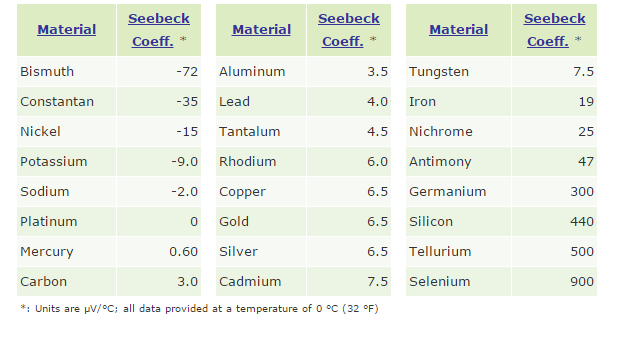
\includegraphics[width=0.7\textwidth]{Seebeckkof.png}
	\caption{Literaturwerte des Seebeckkoeffizienten\footcite{Seebecklit}}
  \label{fig:Seebecklit}
\end{figure}
\begin{table}[H]
  \centering
  \begin{tabular}{c | c | c}
    Material 1 & Material 2 & Resultierender Seeeckkoeffizienten[mV/K]\\ \hline
    Konstantan  & Platin & -0,035\\
    Kalium & Antimon & 0,038\\
    Bismut & Konstantan & -0,037
  \end{tabular}
  \caption{Einige mögliche Kombinationen die ein $\alpha_{AB}\approx m$ ergeben}
  \label{tab:thermobeispiele}
\end{table}
Das Vorzeichen des Seeeckkoeffizienten ist dabei nicht entscheidend, weil keine bestimmte Messrichtung vorgegeben war und bei Umpolung des Messgeräts der gleiche Wert mal $-1$ heraus kommt.

So lässt sich sagen, dass die Messung zwar gelungen ist, es sind realistische Werte herausgekommen, jedoch reicht dies nicht aus um das Material genau zu bestimmen.